\documentclass{ximera}

%\usepackage{todonotes}

\newcommand{\todo}{}

\usepackage{esint} % for \oiint
\graphicspath{
  {./}
  {ximeraTutorial/}
}

\newcommand{\mooculus}{\textsf{\textbf{MOOC}\textnormal{\textsf{ULUS}}}}

\usepackage{tkz-euclide}
\tikzset{>=stealth} %% cool arrow head
\tikzset{shorten <>/.style={ shorten >=#1, shorten <=#1 } } %% allows shorter vectors

\usetikzlibrary{backgrounds} %% for boxes around graphs
\usetikzlibrary{shapes,positioning}  %% Clouds and stars
\usetikzlibrary{matrix} %% for matrix
\usepgfplotslibrary{polar} %% for polar plots
\usetkzobj{all}
\usepackage[makeroom]{cancel} %% for strike outs
%\usepackage{mathtools} %% for pretty underbrace % Breaks Ximera
\usepackage{multicol}
\usepackage{pgffor} %% required for integral for loops


%% http://tex.stackexchange.com/questions/66490/drawing-a-tikz-arc-specifying-the-center
%% Draws beach ball 
\tikzset{pics/carc/.style args={#1:#2:#3}{code={\draw[pic actions] (#1:#3) arc(#1:#2:#3);}}}



\usepackage{array}
\setlength{\extrarowheight}{+.1cm}   
\newdimen\digitwidth
\settowidth\digitwidth{9}
\def\divrule#1#2{
\noalign{\moveright#1\digitwidth
\vbox{\hrule width#2\digitwidth}}}





\newcommand{\RR}{\mathbb R}
\newcommand{\R}{\mathbb R}
\newcommand{\N}{\mathbb N}
\newcommand{\Z}{\mathbb Z}

\newcommand{\sagemath}{\textsf{SageMath}}


%\renewcommand{\d}{\,d\!}
\renewcommand{\d}{\mathop{}\!d}
\newcommand{\dd}[2][]{\frac{\d #1}{\d #2}}
\newcommand{\pp}[2][]{\frac{\partial #1}{\partial #2}}
\renewcommand{\l}{\ell}
\newcommand{\ddx}{\frac{d}{\d x}}

\newcommand{\zeroOverZero}{\ensuremath{\boldsymbol{\tfrac{0}{0}}}}
\newcommand{\inftyOverInfty}{\ensuremath{\boldsymbol{\tfrac{\infty}{\infty}}}}
\newcommand{\zeroOverInfty}{\ensuremath{\boldsymbol{\tfrac{0}{\infty}}}}
\newcommand{\zeroTimesInfty}{\ensuremath{\small\boldsymbol{0\cdot \infty}}}
\newcommand{\inftyMinusInfty}{\ensuremath{\small\boldsymbol{\infty - \infty}}}
\newcommand{\oneToInfty}{\ensuremath{\boldsymbol{1^\infty}}}
\newcommand{\zeroToZero}{\ensuremath{\boldsymbol{0^0}}}
\newcommand{\inftyToZero}{\ensuremath{\boldsymbol{\infty^0}}}



\newcommand{\numOverZero}{\ensuremath{\boldsymbol{\tfrac{\#}{0}}}}
\newcommand{\dfn}{\textbf}
%\newcommand{\unit}{\,\mathrm}
\newcommand{\unit}{\mathop{}\!\mathrm}
\newcommand{\eval}[1]{\bigg[ #1 \bigg]}
\newcommand{\seq}[1]{\left( #1 \right)}
\renewcommand{\epsilon}{\varepsilon}
\renewcommand{\phi}{\varphi}


\renewcommand{\iff}{\Leftrightarrow}

\DeclareMathOperator{\arccot}{arccot}
\DeclareMathOperator{\arcsec}{arcsec}
\DeclareMathOperator{\arccsc}{arccsc}
\DeclareMathOperator{\si}{Si}
\DeclareMathOperator{\proj}{\vec{proj}}
\DeclareMathOperator{\scal}{scal}
\DeclareMathOperator{\sign}{sign}


%% \newcommand{\tightoverset}[2]{% for arrow vec
%%   \mathop{#2}\limits^{\vbox to -.5ex{\kern-0.75ex\hbox{$#1$}\vss}}}
\newcommand{\arrowvec}{\overrightarrow}
%\renewcommand{\vec}[1]{\arrowvec{\mathbf{#1}}}
\renewcommand{\vec}{\mathbf}
\newcommand{\veci}{{\boldsymbol{\hat{\imath}}}}
\newcommand{\vecj}{{\boldsymbol{\hat{\jmath}}}}
\newcommand{\veck}{{\boldsymbol{\hat{k}}}}
\newcommand{\vecl}{\boldsymbol{\l}}
\newcommand{\uvec}[1]{\mathbf{\hat{#1}}}
\newcommand{\utan}{\mathbf{\hat{t}}}
\newcommand{\unormal}{\mathbf{\hat{n}}}
\newcommand{\ubinormal}{\mathbf{\hat{b}}}

\newcommand{\dotp}{\bullet}
\newcommand{\cross}{\boldsymbol\times}
\newcommand{\grad}{\boldsymbol\nabla}
\newcommand{\divergence}{\grad\dotp}
\newcommand{\curl}{\grad\cross}
%\DeclareMathOperator{\divergence}{divergence}
%\DeclareMathOperator{\curl}[1]{\grad\cross #1}
\newcommand{\lto}{\mathop{\longrightarrow\,}\limits}

\renewcommand{\bar}{\overline}

\colorlet{textColor}{black} 
\colorlet{background}{white}
\colorlet{penColor}{blue!50!black} % Color of a curve in a plot
\colorlet{penColor2}{red!50!black}% Color of a curve in a plot
\colorlet{penColor3}{red!50!blue} % Color of a curve in a plot
\colorlet{penColor4}{green!50!black} % Color of a curve in a plot
\colorlet{penColor5}{orange!80!black} % Color of a curve in a plot
\colorlet{penColor6}{yellow!70!black} % Color of a curve in a plot
\colorlet{fill1}{penColor!20} % Color of fill in a plot
\colorlet{fill2}{penColor2!20} % Color of fill in a plot
\colorlet{fillp}{fill1} % Color of positive area
\colorlet{filln}{penColor2!20} % Color of negative area
\colorlet{fill3}{penColor3!20} % Fill
\colorlet{fill4}{penColor4!20} % Fill
\colorlet{fill5}{penColor5!20} % Fill
\colorlet{gridColor}{gray!50} % Color of grid in a plot

\newcommand{\surfaceColor}{violet}
\newcommand{\surfaceColorTwo}{redyellow}
\newcommand{\sliceColor}{greenyellow}




\pgfmathdeclarefunction{gauss}{2}{% gives gaussian
  \pgfmathparse{1/(#2*sqrt(2*pi))*exp(-((x-#1)^2)/(2*#2^2))}%
}


%%%%%%%%%%%%%
%% Vectors
%%%%%%%%%%%%%

%% Simple horiz vectors
\renewcommand{\vector}[1]{\left\langle #1\right\rangle}


%% %% Complex Horiz Vectors with angle brackets
%% \makeatletter
%% \renewcommand{\vector}[2][ , ]{\left\langle%
%%   \def\nextitem{\def\nextitem{#1}}%
%%   \@for \el:=#2\do{\nextitem\el}\right\rangle%
%% }
%% \makeatother

%% %% Vertical Vectors
%% \def\vector#1{\begin{bmatrix}\vecListA#1,,\end{bmatrix}}
%% \def\vecListA#1,{\if,#1,\else #1\cr \expandafter \vecListA \fi}

%%%%%%%%%%%%%
%% End of vectors
%%%%%%%%%%%%%

%\newcommand{\fullwidth}{}
%\newcommand{\normalwidth}{}



%% makes a snazzy t-chart for evaluating functions
%\newenvironment{tchart}{\rowcolors{2}{}{background!90!textColor}\array}{\endarray}

%%This is to help with formatting on future title pages.
\newenvironment{sectionOutcomes}{}{} 



%% Flowchart stuff
%\tikzstyle{startstop} = [rectangle, rounded corners, minimum width=3cm, minimum height=1cm,text centered, draw=black]
%\tikzstyle{question} = [rectangle, minimum width=3cm, minimum height=1cm, text centered, draw=black]
%\tikzstyle{decision} = [trapezium, trapezium left angle=70, trapezium right angle=110, minimum width=3cm, minimum height=1cm, text centered, draw=black]
%\tikzstyle{question} = [rectangle, rounded corners, minimum width=3cm, minimum height=1cm,text centered, draw=black]
%\tikzstyle{process} = [rectangle, minimum width=3cm, minimum height=1cm, text centered, draw=black]
%\tikzstyle{decision} = [trapezium, trapezium left angle=70, trapezium right angle=110, minimum width=3cm, minimum height=1cm, text centered, draw=black]


\title{Abstracting}

\begin{document}

\begin{abstract}
%Stuff can go here later if we want!
\end{abstract}

\maketitle

\begin{sectionOutcomes}

After completing this section, students should understand relations and functions as mathematical tools. 

\begin{itemize}
\item Students .
\item Students .
\end{itemize}

\end{sectionOutcomes}




\textbf{Abstracting} \\
In a family tree, people are connected in many ways.  We have chosen one here. Once you pick a connection rule to follow, then you can list valid pairs of persons - pairs in the relation.  You can also pick pairs that are not valid, are not in the relation.  But, in the end, all we are doing is citing a connection between two sets of things.  In the Totman case, the two sets are both the family members. Other situations might also have this same structure. Noticing this same relational structure with other things is called abstracting.

You might imagine replacing all of the people in the Totman diagram with tomato plants.  The dashed line segments might indicate grafting different plants, while solid might mean a plant grown from seeds resulting from the graft. 

Now we have different situations with similar characteristics. Our mathematics is describing this shared structure. Other situations we investigate with our science might share this common relationship.  In this way our mathematics allows us to see how different situations might share common characteristics. Any thoughts we develop about one could then easily be translated to the other situations. We call this \textbf{abstracting}.

We abstract every day.  We see common connections, borrow language, and make analogies to help others understand the structure we see. We see the relation structure in just about everything, from family trees, to growing plants, to football teams. 





\begin{example}
\quad \\
\textbf{Try It Yourself}

\begin{image}
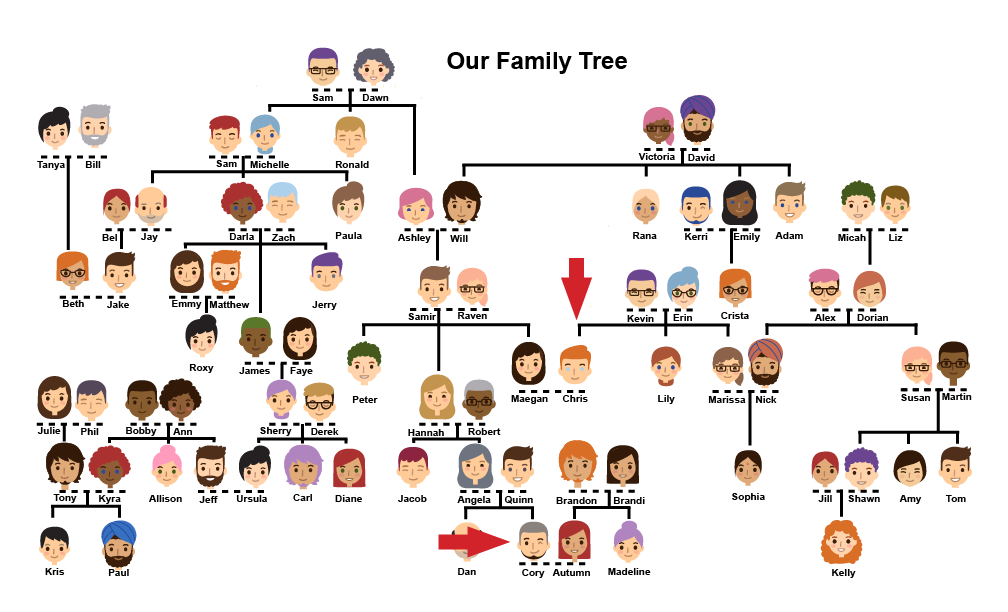
\includegraphics{pics/Chris_Cory_arrow.png}
\end{image}

Is (Chris, Cory) $\in$ Totman Relation?
\begin{multipleChoice}
\choice{Yes}
\choice[correct]{No}
\end{multipleChoice}
\begin{feedback}
The only path from Cory to Chris crosses over the full dashed line segment at the marriage of Meagan and Chris.
\end{feedback}


\end{example}
\quad \\




\begin{example}
\quad \\
\textbf{Try It Yourself}

\begin{image}
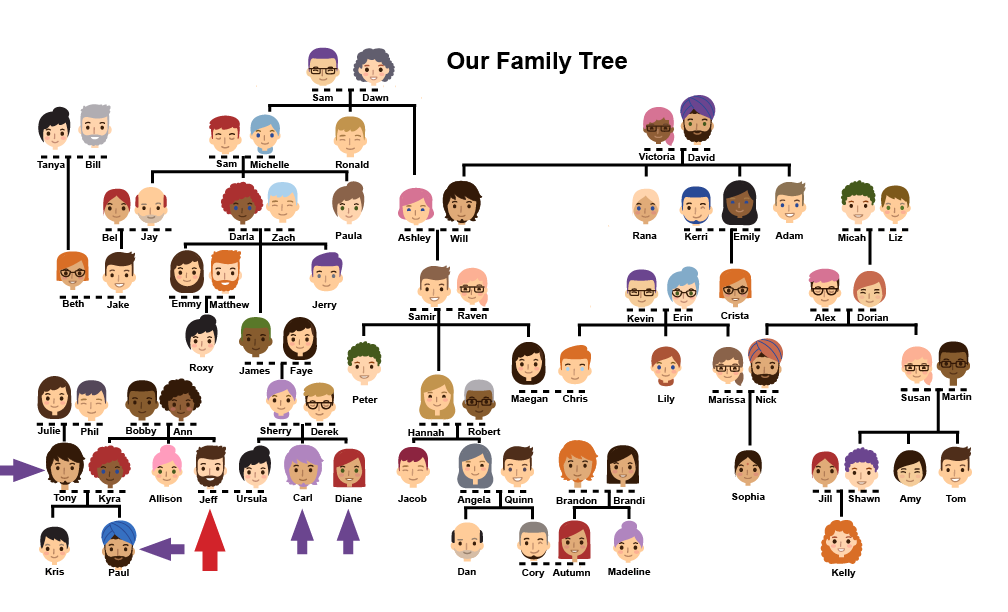
\includegraphics{pics/Jeff_arrow.png}
\end{image}

If (Jeff, person) $\in$ Totman Relation, then who could the person be?
\begin{multipleChoice}
\choice{Carl}
\choice{Tony}
\choice[correct]{Paul}
\choice{Diane}
\end{multipleChoice}
\begin{feedback}
The path to Paul is the only one of the four that doesn't cross over a full dashed line segment.
\end{feedback}


\end{example}
\quad \\





\begin{example} 
\quad \\
Let's consider Franklin High School's swim team. There are 7 students on the team.

\begin{center}
\[
\begin{array}{|c|c|}
\hline
\textbf{NAME} & \textbf{AGE} \\\hline
Sally & 16 \\\hline
Jim & 18 \\\hline
Sarah & 16 \\\hline
Taja & 17 \\\hline
Jacob & 17 \\\hline
Dawn & 18 \\\hline
Kacey & 17 \\\hline
Corey & 17 \\\hline
\end{array}
\]
\end{center}

Sets: students and students.

Relation: two students are related to each other if they are the same age. We'll call this relation SameAge.

Mathematics: The ordered pair (person 1, person 2) is in SameAge if person 2 is the same age as person 1. 

(Sally, Sarah) is an ordered pair in SameAge.  (Taja, Dawn) is not an ordered pair in SameAge.

Is SameAge reflexive?  
\begin{multipleChoice}
\choice[correct]{Yes}
\choice{No}
\end{multipleChoice}
\begin{feedback}
A person is the same age as himself or herself. The pair (person1, person1) is \textbf{ALWAYS} in SameAge.
\end{feedback}
\quad \\

Is SameAge symmetric? 
\begin{multipleChoice}
\choice[correct]{Yes}
\choice{No}
\end{multipleChoice}
\begin{feedback}
If (person1, person2) $\in$ SameAge, then person1 and person2 are the same age, which means that  (person1, person2) $\in$ SameAge - \textbf{ALWAYS}.
\end{feedback}
\quad \\

Is SameAge transitive? 
\begin{multipleChoice}
\choice[correct]{Yes}
\choice{No}
\end{multipleChoice}
\begin{feedback}
If (person1, person2) $\in$ SameAge and (person2, person3) $\in$ SameAge, than (person1, person3) $\in$ SameAge. \textbf{ALWAYS}.  
\end{feedback}


\end{example}
\quad \\





\begin{example} 
\quad \\
Let's consider Franklin High School's swim team. There are 7 students on the team. 

\begin{center}
\[
\begin{array}{|c|c|}
\hline
\textbf{NAME} & \textbf{AGE} \\\hline
Sally & 16 \\\hline
Jim & 18 \\\hline
Sarah & 16 \\\hline
Taja & 17 \\\hline
Jacob & 17 \\\hline
Dawn & 18 \\\hline
Kacey & 17 \\\hline
Corey & 17 \\\hline
\end{array}
\]
\end{center}




Sets: students and students.

Relation: students are older and younger than each other.

Mathematics: describe this structure with ordered pairs for a relation called Older. The ordered pair (person 1, person 2) is in Older if person 2 is older than person 1. 

(Sally, Dawn) is an ordered pair in Older.  (Taja, Sarah) is not an ordered pair in Older.

Is Older reflexive? 
\begin{multipleChoice}
\choice{Yes}
\choice[correct]{No}
\end{multipleChoice}
\begin{feedback}
A person is not older than himself or herself. The pair (person1, person1) cannot be in Older. 
\end{feedback}
\quad \\

Is Older symmetric? 
\begin{multipleChoice}
\choice{Yes}
\choice[correct]{No}
\end{multipleChoice}
\begin{feedback}
(Sally, Dawn) $\in$ Older, but (Dawn, Sally) is not since Sally is not older than Dawn.
\end{feedback}
\quad \\

Is Older transitive? 
\begin{multipleChoice}
\choice[correct]{Yes}
\choice{No}
\end{multipleChoice}
\begin{feedback}
If (person1, person2) $\in$ Older and (person2, person3) $\in$ Older, than (person1, person3) $\in$ Older. \textbf{ALWAYS}.   
\end{feedback}
                   
\end{example}
\quad \\                                                                                     



                                                                                                            
Let's change the Totman connection to be "a relative". Two people in the Totman family tree are relatives of each other if there is a path which includes AT MOST one full dashed line segment. It can include any number of solid or half-dashed pieces. Let's call this the Totman-Rel relation.



\begin{exercise}
\quad \\
\begin{center}
\begin{image}
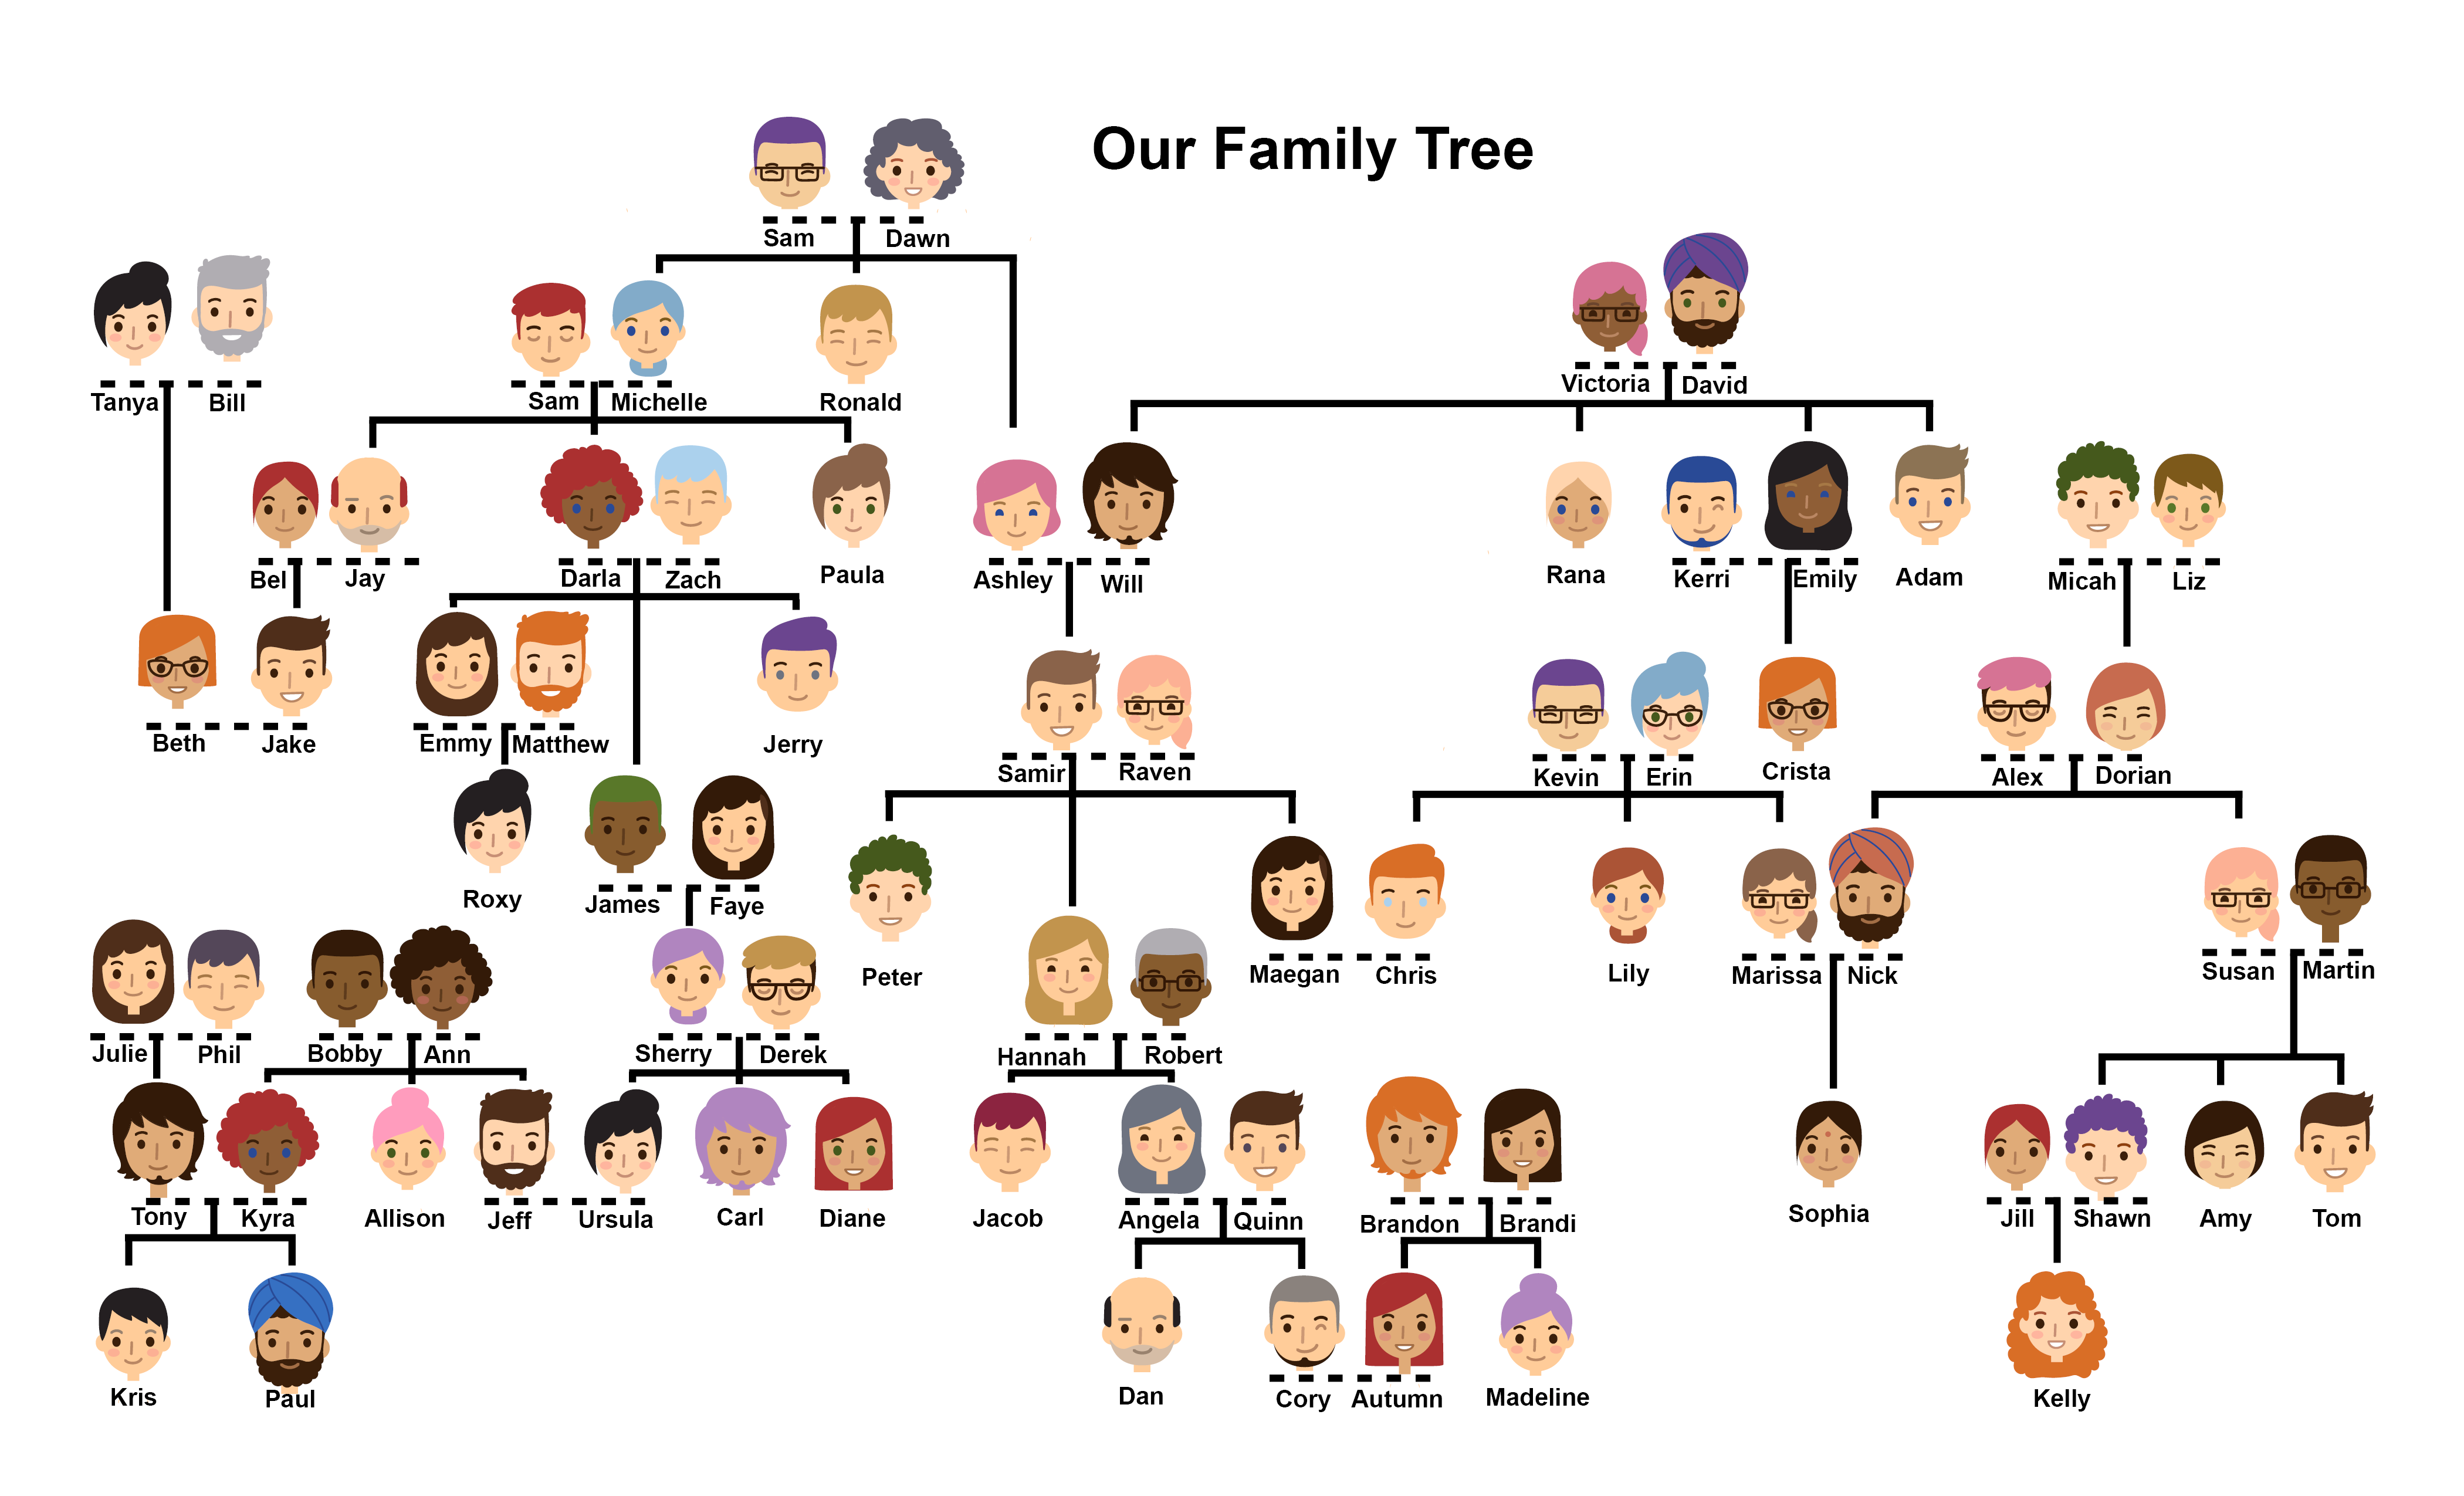
\includegraphics{Totman_Family_Tree.png}
\end{image}
\end{center}


\begin{problem} Is (Ashley, Victoria) $\in$ Totman-Rel ? \wordChoice{\choice[correct]{Yes} \choice{No}}
\begin{feedback}
Ashley-Will-Victoria includes at most one full dashed line segment, the one representing the marriage of Ashley and Will.
\end{feedback}
\end{problem}


\begin{problem} Is (Ashley, Crista) $\in$ Totman-Rel ?  \wordChoice{\choice[correct]{Yes} \choice{No}}
\begin{feedback}
Ashley-Will-Emily-Crista includes at most one full dashed line segment, the one representing the marriage of Ashley and Will.
\end{feedback}
\end{problem}


\begin{problem} Is (Ashley, Kevin) $\in$ Totman-Rel ?  \wordChoice{\choice[correct]{Yes} \choice{No}}
\begin{feedback}
Ashley-Samir-Meagan-Chris-Kevin includes at most one full dashed line segment, the one representing the marriage of Maegan and Chris.
\end{feedback}
\end{problem}

\begin{problem} Is (Ashley, Alex) $\in$ Totman-Rel ?  \wordChoice{\choice{Yes} \choice[correct]{No}}
\begin{feedback}
Ashley-Samir-Meagan-Chris-Marissa-Nick-Alex includes two full dashed line segments, the one representing the marriage of Maegan and Chris, and the one representing the marriage of Marissa and Nick.
\end{feedback}
\end{problem}

\begin{problem} Is (Ashley, Zach) $\in$ Totman-Rel ?  \wordChoice{\choice[correct]{Yes} \choice{No}}
\begin{feedback}
Ashley-Michelle-Daria-Zach includes at most one full dashed line segment, the one representing the marriage of Daria and Zach.
\end{feedback}
\end{problem}

\begin{problem} Does the Totman-Rel relation contain (Ashley, Quinn) ?  \wordChoice{\choice[correct]{Yes} \choice{No}}
\begin{feedback}
Ashley-Samir-Hannah-Angela-Quinn includes at most one full dashed line segment, the one representing the marriage of Angela and Quinn.
\end{feedback}
\end{problem}

\begin{problem} Does the Totman-Rel relation contain (Ashley, Brandi) ?  \wordChoice{\choice[correct]{Yes} \choice{No}}
\begin{feedback}
Ashley-Samir-Hannah-Angela-Cory-Autumn-Brandi includes at most one full dashed line segment, the one representing the marriage of Cory and Autumn.
\end{feedback}
\end{problem}

\begin{problem} Is every pair in the Totman relation also in the Totman-Rel relation?  \wordChoice{\choice[correct]{Yes} \choice{No}}
\begin{feedback}
Every path that doesn't contain a full dashed line segment is a path that contains at most one full dashed line segment.
\end{feedback}
\end{problem}

\begin{problem} Is the Totman-Rel relation symmetric?  \wordChoice{\choice[correct]{Yes} \choice{No}}
\begin{feedback}
Forwards or backwards, the path contains the same number of marriages and full dashed line segments.
\end{feedback}
\end{problem}

\begin{problem} Does the Totman or the Totman-Rel relation contain more pairs?  \wordChoice{\choice{Totman} \choice[correct]{Totman-Rel}}
\begin{feedback}
The Totman-Rel relation contains more, because it contains every path in the Totman relation plus several noted in these answers that would not be in the Totman relation.
\end{feedback}
\end{problem}





\end{exercise}



\begin{remark} \textbf{COMMUNICATION} \\
Eventually, we will juggle many relations. This is going to cause a communication nightmare. We will need more language for our relations just to keep our thoughts organized in our heads.

For one thing, we?ll need official names for the first and second sets/collections.

We?ll names for the relations, so that we know which ones we are talking about.

We?ll invent language to help us as we move deeper into the investigation of relations.

\end{remark}












\end{document}
